% From Replayable Traces to Provenance-Aware Rule Fusion:
% Bounded Auditability Evidence for Reinforcement Learning Policies
% Evidence-aligned manuscript. Claims are bounded to the evaluated prototype,
% tasks, seeds, and execution setup.
\documentclass[11pt,a4paper]{article}

\usepackage{amsmath,amssymb,amsthm}
\usepackage{mathtools}
\usepackage{booktabs}
\usepackage{graphicx}
\usepackage{tikz}
\usetikzlibrary{shapes,arrows,positioning,calc}
\usepackage{hyperref}
\usepackage[numbers,sort&compress]{natbib}
\usepackage{microtype}
\setlength{\emergencystretch}{2em}
\usepackage{enumitem}
\usepackage{caption}
\usepackage{subcaption}

\theoremstyle{definition}
\newtheorem{definition}{Definition}[section]
\newtheorem{protocol}{Protocol}[section]

\title{From Replayable Traces\\ to Provenance-Aware Rule Fusion:\\
Bounded Auditability Evidence for Reinforcement Learning Policies}
\author{Evidence-aligned manuscript\\ synthesised from repository-grounded experiments}
\date{22 September 2026}

\begin{document}
\maketitle

\begin{abstract}
Reinforcement learning auditability is often invoked as a single property.
We argue, and then demonstrate empirically, that it is at least four distinct
properties: whether a recorded execution is intact and replayable, whether a
learned symbol causally changes a decision, whether symbolic rules capture
behaviour shared across agents, and whether those rules can be composed with
visible provenance. Passing one test does not imply passing the others.
We report a bounded end-to-end study that measures each separately and
deliberately reports where tempting inferences fail. In a designed
coordination task, matched-support interventions on the information-bearing
learned symbol changed receiver action probability by $0.997$--$1.000$ across
six seeds. In two benchmark control tasks, eight agents per task were trained
for $300$ episodes each under one shared frozen state symbolizer. Exact
rule-set overlap between two agents reached $0.583$ on the first task but only
$0.050$ on the second; direct measurement of deterministic action agreement on
$10{,}000$ fresh held-out states gave only $51.4\%$ (episode-cluster interval
$50.5\%$--$52.3\%$) for the first pair, rejecting overlap as a proxy for
behavioural consensus. A provenance-aware fusion procedure that records
sources, conflicts, blind spots, and fallbacks achieved mean returns of
$205.96$ versus $163.65$ for the best single agent on the first task and
$-443.37$ versus $-500.00$ on the second, with $95.7\%$ rule coverage and
$89.2\%$ conflict on the second task. Arbitration proved fragile: random
selection among available source rules unexpectedly outperformed the tested
deterministic arbiters, while uniform random actions did not. Value-based
composition diagnostics failed quality checks and are reported separately.
The evidence supports the existence of replayable, provenance-visible
rule composition in these settings; generality, universal causal explanation,
and complete auditability of arbitrary training remain unproven.
\end{abstract}

\noindent\textbf{Scope statement.}
Every number in this paper is tied to the evaluated prototype, the two
benchmark tasks, the stated seeds and sample sizes, and the recorded software
and hardware setup. The paper claims bounded existence, not universality.

\tableofcontents
\newpage

%======================================================================
\section{Introduction: starting from the naive picture}
%======================================================================

\subsection{Scenario}

Consider a team that has trained several reinforcement learning agents and is
asked, after the fact, to explain what happened. The most natural first
proposal is disarmingly simple: keep a complete log of states, actions, and
rewards; compress repeated patterns into grammar-like rules; check that the
log has not been altered; and replay it in the environment. If each step
checks out, the training run is declared auditable. If the induced rules
overlap across agents, they are declared a shared policy core. If the rules
can be merged, the merger is declared an interpretable composition. Each
inference feels like a small step from the previous one.

This paper begins from that naive picture on purpose, because the project
described here began there too. The contribution of the work is not that the
naive picture was confirmed. It is that each of its steps was instrumented,
stress-tested, and in several cases refuted, and that what survived is a
narrower but defensible set of mechanisms with explicit failure modes.

\subsection{Why the obvious approaches do not suffice}

Three limitations of the naive picture structured the entire investigation.

First, \emph{recording is not replaying, and replaying is not explaining.}
A hash chain detects modification of a record; it does not prove the recorded
transition actually occurred in the claimed environment, nor does it identify
why a neural network selected an action. Early in this project, integrity
checks passed while the environment-replay check they actually required had
not yet been built. The lesson, formalised in Section~\ref{sec:methods}, is
that integrity, transition fidelity, and causal attribution are separate
quantities requiring separate estimators.

Second, \emph{compression is not generalisation.} A grammar that reconstructs
a training trajectory exactly may cover almost none of the states encountered
at deployment, or may predict the wrong action where it does cover. The first
pilot reported here induced rules that agreed with the source policy on
$100\%$ of a $0.4\%$ covered subset while the constrained policy lost nearly
$380$ return points. Lexical symbol reduction of $28.6\%$ coexisted with a
serialized artifact $1.80\times$ larger than the original trace. Both episodes
are reported in detail because they are the reason the final design separates
a lossless trajectory codec from a state-conditioned rule bank and evaluates
them with disjoint metrics.

Third, \emph{syntactic overlap is not behavioural consensus, and coverage is
not arbitration.} Two agents may share many identical symbolic rules yet
choose different actions on the same fresh states; a fusion procedure may
cover $95.7\%$ of decisions yet be decided almost entirely by how it resolves
the $89.2\%$ that conflict. Both phenomena occurred in this study, and both
are now central results rather than footnotes.

\subsection{Problem and objective}

The problem addressed is therefore not ``make reinforcement learning
auditable'' as a slogan. It is: for specified artifacts and specified
executions, which audit questions can be answered, with what estimator, under
what stated conditions, and where do the natural generalisations break? The
objective is a bounded existence claim: exhibit a workflow that exposes
replayable execution records, tests a learned symbol's causal influence in a
designed communication task, and composes learned state--action rules while
identifying their sources, conflicts, and uncovered states --- and document
the boundaries with the same care as the mechanisms.

\subsection{Challenges: why direct reuse fails}

Four challenges prevented direct reuse of standard components, and each
forced a design decision documented below.

\paragraph{Challenge 1: the observer must not perturb training.}
Any instrumentation that changes optimisation invalidates the very execution
it claims to record. The first implementation accidentally did so twice: a
serialised wrapper label leaked into the weight hash, and a grammar sidecar
counter leaked into the update ledger. Both produced spurious mismatch
alarms. The fix was to hash only optimisation-relevant tensors and to define
a normalised core-update hash excluding sidecar metadata
(Section~\ref{sec:methods}).

\paragraph{Challenge 2: the symbolizer is itself a confounder.}
When each agent fits its own state discretizer, identical bin labels need not
denote identical raw-state regions; the largest observed edge difference was
$0.157$ observation units. Overlap statistics computed under mismatched
discretizers conflate representation agreement with policy agreement. The fix
was a single pooled frozen symbolizer per task, fitted from separate
random-policy calibration rollouts before any scored training.

\paragraph{Challenge 3: the value baseline may be uninformative.}
A fitted action-value model with mean absolute error above $40$ return units
on held-out transitions, whose greedy actions disagree with the actor on
nearly two thirds of states and collapse to a single action on an entire
diagnostic set, cannot adjudicate between composition methods. The study
therefore demoted its value-based comparator to a diagnostic-only role rather
than suppressing it.

\paragraph{Challenge 4: the communication task may not require
communication.}
In the early coordination design, the payoff structure made the same joint
action optimal regardless of the private signal, so the receiver could attain
the optimum without any message; the proposed blind-receiver control left the
image pathway unmasked; and the discrete codebook was bypassed by a
continuous encoder path. Each defect made symbols unnecessary by
construction. The fix was a decision-relevant payoff redesign with jointly
masked private pathways, reported as a failure-to-redesign narrative in
Section~\ref{sec:failures}.

\subsection{Method components mapped to challenges}

The final workflow contains five components, each answering one challenge:
(i)~a frozen shared symbolizer and admitted rule bank with support and
confidence thresholds; (ii)~a lossless trajectory codec kept metrically
separate from the rule bank; (iii)~a provenance-aware fusion procedure with
explicit conflict, blind-spot, and fallback records bound by a hash chain;
(iv)~an independent environment-replay validator comparing full transition
tuples; and (v)~a held-out behavioural-agreement test on fresh raw states
plus matched arbitration and value-diagnostic controls.

\subsection{Contributions}

\begin{enumerate}[leftmargin=2em]
\item A provenance-aware rule-fusion prototype with explicit source
attribution, conflict arbitration, blind-spot detection, and fallback
logging, evaluated on matched reset seeds with paired uncertainty intervals.
\item Shared-symbolizer multi-seed measurements of exact rule overlap on two
tasks, paired with a fresh-state behavioural-agreement test that refutes
overlap as a consensus proxy in this setting.
\item End-to-end artifact checks covering hash-linked records, source-rule
resolution, optimisation-ledger equivalence, and exact environment-transition
replay under the recorded setup, with byte-level provenance accounting.
\item A causal-intervention result for learned symbols in a designed
coordination task, kept strictly distinct from state--action rule fusion and
from general natural-language interpretability.
\item A documented failure record --- coverage collapse, serialization
inversion, arbitration instability including an unexpected random-arbitration
advantage, and value-baseline failure --- with the design changes and the
reasons each failure occurred.
\end{enumerate}

%======================================================================
\section{From failures to fixes: the experimental trajectory}
\label{sec:failures}
%======================================================================

This section honours the requested shallow-to-deep order: it narrates what
was tried, what failed, why it failed, and what replaced it, before any
formalism. Readers who prefer the final formalism first may skip to
Section~\ref{sec:methods}; nothing there depends on this narrative, but the
narrative explains why the formalism looks the way it does.

\paragraph{Failure 1: the legacy prototype could not run as specified.}
The inherited implementation failed at first contact: an unexpected
constructor argument, double environment resets without fixed seeds, ignored
truncation flags despite a $500$-step time limit, one-step and windowed rule
counts conflated under a single denominator without reward weighting, a
greedy bigram-substitution routine presented as canonical SEQUITUR without
digram-uniqueness or rule-utility enforcement, lossy truncation of the start
production, substring-based provenance instead of occurrence provenance, and a
coverage test that skipped uninitialised abstractions without counting
failures and never re-executed the environment. \emph{Reason:} operational
plumbing had been mistaken for a scientific instrument. \emph{Fix:} a
validated execution path separating state--action production induction, an
exact pair-substitution codec for complete transition records, held-out
coverage and agreement tests, and constrained-policy comparisons with
explicit fallbacks; the legacy code was retained only as a labelled wrapper.

\paragraph{Failure 2: constraints that helped one seed destroyed another.}
With admission at support at least $8$ and confidence at least $0.90$, the
seed-$11$ constrained policy covered $0.4\%$ of held-out steps and scored
$121.3$ against a $500.0$ baseline, while seed $29$ gained modestly. Lowering
confidence to $0.70$ raised coverage to $75.6\%$ and $56.4\%$ but lowered
agreement to $59.9\%$ and $74.2\%$, with deltas of $-330.4$ and $+17.0$.
\emph{Reason:} a global action mask and a low-coverage lookup confuse
conditional precision with policy quality; training coverage does not imply
deployment coverage. \emph{Fix:} the constrained-training arm was abandoned
as a performance claim; the surviving artifact is the fusion procedure of
Section~\ref{sec:methods}, which never acts without recording agreement,
single-source coverage, conflict, or blind spot, and which selects its
fallback from training metadata only.

\paragraph{Failure 3: compression that expanded the artifact.}
Sixteen pair productions reduced lexical symbols from $9{,}178{,}724$ to
$6{,}558{,}026$ (ratio $0.715$) with exact round-trip, yet the readable
artifact was $110.5$~MB against a $61.3$~MB original ($1.80\times$).
\emph{Reason:} string references cost more bytes than the symbols they save.
\emph{Fix:} integer terminal identifiers with exact offsets and gzip
serialization, plus an honest comparison: the compact grammar archive is
$78.2\%$ smaller than raw text but $8.4\%$ larger than plain gzip of the same
trace. Grammar structure is therefore reported as provenance value, not as a
storage win. Per-round two-part description lengths rose monotonically in
relative terms ($0.513$ to $0.575$), confirming that the inducer does not
optimise the code-length score.

\paragraph{Failure 4: the audit ledger indicted itself.}
Baseline and observer-only arms matched on weights and traces yet mismatched
on the update ledger. \emph{Reason:} the ledger had absorbed a grammar sidecar
counter unrelated to optimisation. \emph{Fix:} sidecar removal and a
normalised core-update hash; the correction is retained in the record rather
than rewritten.

\paragraph{Failure 5: the symbolizer confound.}
Seed-specific quantile edges differed by up to $0.157$ units, so identical
symbols could denote different raw regions. \emph{Fix:} one pooled frozen
symbolizer per task from $24$ random-policy episodes per seed, shared across
all seeds and arms.

\paragraph{Failure 6 (central negative): overlap without agreement.}
Under the shared symbolizer, the seed-$11$ versus seed-$29$ exact rule
overlap reached $0.583$ with zero same-condition action conflicts, yet
deterministic action agreement on $10{,}000$ fresh raw states was $51.4\%$,
with an episode-cluster interval of $50.5\%$--$52.3\%$.
\emph{Reason:} Jaccard counts shared symbolic conditions under the training
occupancy; agreement measures action equality under held-out occupancy, where
the two source policies in fact occupy different return regimes (means
$500.0$ versus $130.9$). Syntax statistics cannot stand in for behavioural
measurement.

\paragraph{Failure 7 (open finding): arbitration dominates coverage.}
On the second task, fusion covered $95.7\%$ of $44{,}376$ decisions with only
$4.3\%$ blind spots, yet $89.2\%$ of decisions conflicted. Confidence-only
arbitration tied the primary rule ($-444.49$ versus $-443.37$); reward-only,
support-first, and ensemble-deferral variants all scored $-500.00$; random
selection among available source rules scored $-187.02$ on one stream and
$-194.10$ to $-206.17$ across five independent streams (mean $-198.82$),
while uniform random actions averaged $-498.71$. \emph{Reason, partial:}
$1{,}575$ of $1{,}694$ rules carry identical mean reward $-1.0$, collapsing
reward-ranked arbitration to tie order; confidence ranking is simply not a
validated resolver here. The mechanism of the random-rule advantage ---
a state-conditioned mixture over source rules --- is identified as a policy
class but not as an explanation; source-frequency and occupancy decomposition
remain future work.

\paragraph{Failure 8: the value baseline failed its own checks.}
The fitted value comparator scored $9.34$ against $163.65$ on the first task,
matched the actor ensemble on only $35.27\%$ of $31{,}563$ held-out states,
selected a single action on all $50{,}000$ diagnostic states on the second
task, and exhibited scalar value correlation ($0.652$) alongside near-total
greedy-action divergence. \emph{Reason:} large prediction error combined with
extrapolation outside source-policy support. \emph{Fix:} demotion to a
diagnostic-only role, reported separately so it cannot contaminate the fusion
result.

\paragraph{Failure 9: a communication task that needed no communication.}
Source review showed the original coordination payoff made the same joint
action optimal for both parities, the blind control masked only the label
while the image encoder retained parity information, a reserved index lay
outside the embedding range, the codebook was bypassed by a straight-through
continuous path, and an opponent-prediction branch was degenerately solvable
by copying. \emph{Fix:} a parity-critical payoff with opposed optima and
preserved betrayal temptation, joint masking of label and image pathways with
a neutral constant, corrected index handling, straight-through codebook
wiring with perplexity reporting, and a staged gate (diversity, positive
control, necessity, generalisation, causality, channel exclusivity) with
pre-registered verdicts. The surviving causal result in Section~\ref{sec:results}
comes from the redesigned task and is bounded to it.

%======================================================================
\section{Methods}
\label{sec:methods}
%======================================================================

\subsection{Problem formulation}

Let $s \in \mathcal{S} \subseteq \mathbb{R}^{d}$ be a raw state and
$a \in \mathcal{A}$ a discrete action with $|\mathcal{A}| \in \{2,3\}$.
A stochastic policy $\pi_{\theta}(a \mid s)$ is trained by a policy-gradient
procedure; a deterministic evaluation policy uses
$\hat{a}(s) = \arg\max_{a} \pi_{\theta}(a \mid s)$.
An execution of $E$ episodes yields a transition record
$\tau = \{(s_t, a_t, r_t, s'_t, d_t, u_t, e_t)\}_{t=1}^{T}$ with reward,
next state, termination, truncation, and reset-seed fields. Three claims are
distinguished from the outset: integrity of $\tau$, fidelity of replay of
$\tau$ in the environment, and agreement of derived rules with $\hat{a}$ on
specified state distributions. No single metric is allowed to certify more
than one claim.

Falsifiable predictions registered before the corresponding results are:
(P1)~baseline and observer-only arms produce identical optimisation tensors
and traces; (P2)~exact environment replay matches every transition tuple;
(P3)~exact rule overlap overstates held-out action agreement for the
examined pair; (P4)~fusion return and arbitration rank are sensitive to the
conflict resolver under matched reset seeds. Value-based composition carries
no registered prediction because its diagnostics failed gate checks.

\subsection{Central mechanism: symbolizer, rule bank, and fusion}

\paragraph{Shared frozen symbolizer.}
Per task, a calibration pool of random-policy episodes from every seed
induces per-dimension empirical quantile edges with $B=4$ bins, frozen before
scored training. The symbolizer is
\begin{equation}
\phi(s) = \big(q_1(s_1), \dots, q_d(s_d)\big) \in \mathcal{C},
\qquad |\mathcal{C}| = B^{d},
\label{eq:symbolizer}
\end{equation}
where $q_j$ is the quantile-bin index of coordinate $j$.
All agents, arms, and evaluations within a task share $\phi$.

\paragraph{Admitted state--action rules.}
For symbolic condition $c \in \mathcal{C}$ and action $a$, let
$n(c,a)$ be the training-occupancy count and
$n(c) = \sum_{a} n(c,a)$. Support and confidence are
\begin{equation}
\mathrm{supp}(c,a) = n(c,a),
\qquad
\mathrm{conf}(c,a) = n(c,a) / n(c).
\label{eq:rules}
\end{equation}
The admitted bank for source $i$ is
$\mathcal{R}_i = \{(c,a) : \mathrm{supp} \ge 8,\ \mathrm{conf} \ge 0.70\}$,
each entry annotated with mean reward, source-step references, and grammar
hashes. The bank is distinct from the lossless trajectory codec, which encodes
complete transition records and is evaluated only by exact round-trip and
explicit two-part code length.

\paragraph{Overlap and agreement.}
For banks $\mathcal{R}_i,\mathcal{R}_j$ over $(c,a)$ productions, syntactic
overlap is the Jaccard statistic
\begin{equation}
J(\mathcal{R}_i,\mathcal{R}_j)
= \frac{|\mathcal{R}_i \cap \mathcal{R}_j|}
{|\mathcal{R}_i \cup \mathcal{R}_j|}.
\label{eq:jaccard}
\end{equation}
Behavioural agreement on a held-out raw-state distribution $Q$ is the
estimand
\begin{equation}
A_{ij} = \mathbb{E}_{s \sim Q}\big[\mathbf{1}\{\hat{a}_i(s)=\hat{a}_j(s)\}\big],
\label{eq:agreement}
\end{equation}
estimated by pooled and episode-cluster-balanced means with percentile
bootstrap intervals. Equation~\eqref{eq:jaccard} is a syntax statistic;
Equation~\eqref{eq:agreement} is a behaviour statistic. The paper tests,
rather than assumes, any relation between them.

\paragraph{Provenance-aware fusion.}
At raw state $s$, each source contributes at most one candidate via its own
frozen symbolizer and bank. Let $\mathcal{K}(s)$ be the multiset of available
candidates. The decision rule is
\begin{equation}
\delta(s) =
\begin{cases}
\text{agree}(s), & |\mathcal{K}(s)| \ge 2\ \text{and unanimous},\\
\text{single}(s), & |\mathcal{K}(s)| = 1\ \text{up to multiplicity},\\
\rho(\mathcal{K}(s)), & \text{conflicting candidates},\\
f(s), & \mathcal{K}(s) = \varnothing\ \text{(blind spot)},
\end{cases}
\label{eq:fusion}
\end{equation}
where $\rho$ is the declared arbitration order
(confidence, then support, then mean reward, then source-seed tiebreak) and
$f$ is a fallback source policy selected from training-return metadata only,
without using evaluation returns. Every decision records candidate rule
identifiers, source-run references, grammar digests, support, confidence,
reward statistics, the arbitration outcome or fallback identity, and a
hash-chain link. Ablations replace $\rho$ with confidence-only,
reward-only, support-first, uniform-random-over-$\mathcal{K}(s)$, and
ensemble-deferral variants on identical reset seeds.

\begin{protocol}[Fusion evaluation]
Fix $100$ reset seeds shared by every policy. Roll out each policy
deterministically. Report mean, median, per-episode returns, paired
differences against the best single source with $95\%$ percentile bootstrap
intervals, and the decision mix (covered, conflicting, blind-spot counts and
step totals). Repeat stochastic arbiters over five independent selector
streams; run a matched uniform-random-action control over the same seeds.
\end{protocol}

The protocol state machine has four non-terminal decision states
(agreement, single-source, conflict, blind spot) plus terminal logging and
verification states; more than eight operator steps are intentionally kept
outside the manuscript and retained in the internal audit package.

\subsection{Artifact integrity, provenance binding, and replay}

Let $h_t$ chain block $t$ of the decision or transition log. The binding
predicate is
\begin{equation}
V_{\mathrm{chain}} = \bigwedge_{t} \big[h_t = H(h_{t-1} \Vert x_t)\big],
\label{eq:chain}
\end{equation}
with $x_t$ the canonical block payload and $H$ the digest function.
Source-rule resolution requires
\begin{equation}
V_{\mathrm{prov}}(t) = \big[\mathrm{ref}_t \in \mathcal{R}_{i(t)}
\ \wedge\ \mathrm{act}(\mathrm{ref}_t) = a_t
\ \wedge\ \mathrm{stat}(\mathrm{ref}_t) = \widehat{\mathrm{stat}}_t\big],
\label{eq:prov}
\end{equation}
checked for every selected reference. Environment replay requires
\begin{equation}
V_{\mathrm{replay}} = \bigwedge_{t} \big[
\hat{s}_t = s_t\ \wedge\ \hat{s}'_t = s'_t\ \wedge\
\hat{r}_t = r_t\ \wedge\ \hat{d}_t = d_t\ \wedge\ \hat{u}_t = u_t
\big],
\label{eq:replay}
\end{equation}
where hatted quantities are produced by re-executing recorded reset seeds
and actions in an independent environment instance with exact floating-point
comparison. Optimisation-ledger equivalence between baseline and
observer-only arms is asserted only on the normalised core hash excluding
instrumentation sidecars. A tamper probe (single-reward modification) is
expected to fail at the first altered block.

\subsection{Data generation, cohort, and experimental design}

Environments are two fixed discrete-action benchmark tasks with $4$- and
$6$-dimensional observations and $2$ and $3$ actions. The cohort is eight
training seeds per task ($11, 29, 43, 71, 101, 149, 211, 307$), each with
$300$ training episodes per arm across three arms (baseline, observer-only,
constrained), one pooled frozen symbolizer per task from $24$ separate
random-policy calibration episodes per seed, and $100$ matched evaluation
episodes per policy. The behavioural-agreement test uses $100$ fresh episodes
per source on disjoint reset ranges, sampling $5{,}000$ states per occupancy
without replacement and applying both deterministic actors to the same
$10{,}000$ raw states. The coordination-intervention experiment is a separate
six-seed designed task with $600{,}000$ logged decisions, shuffled-message
and no-message controls, and matched-support symbol interventions.

\subsection{Estimators, analysis strategy, and validity}

Point estimates are means, medians, Jaccard values, agreement rates, and
coverage and conflict fractions. Uncertainty is reported by percentile
bootstrap (paired differences on matched seeds; episode-cluster bootstrap for
agreement). The effective sample unit is the episode for returns and the
state for agreement, with cluster adjustment where states nest in episodes.
No multiplicity correction is claimed beyond reporting every retained
comparison. Analysis subsets, smoothing, and exclusions: none beyond the
predeclared admission thresholds and the diagnostic-only demotion of the
value comparator.

Internal validity rests on matched reset seeds, frozen symbolizers, disjoint
calibration, training, and evaluation ranges, and exact ledger and replay
checks. External validity is explicitly bounded to the two tasks, the stated
seeds, and the recorded software and hardware setup; cross-hardware
equivalence and logger honesty are not established. Reliability is
same-configuration determinism (cold reruns matched on all hashes);
statistical reproducibility is interval-based where stochastic arbiters apply.
No human subjects, annotators, or personal data are involved; no ethics-board
approval is claimed or required.

%======================================================================
\section{Results}
\label{sec:results}
%======================================================================

\subsection{Trace integrity and exact replay (P1, P2: supported)}

Across the eight-seed runs, audit records cover $1{,}725{,}655$ trace rows
for the first task and $2{,}544{,}513$ for the second across the three arms;
independent environment replay covers $1{,}122{,}403$ and $1{,}742{,}570$
transitions respectively. Every baseline versus observer-only pair matches
exactly on actor tensors, transition traces, and normalised core-update
hashes; all hash chains validate; every replayed tuple matches on raw state,
next state, reward, termination, and truncation fields. The tamper probe is
rejected at the first altered block. Prediction P1 and P2 are supported
within the recorded setup. This establishes integrity and replayability of
the recorded executions --- not logger honesty, cross-hardware equivalence,
or causal attribution.

\subsection{Shared rules versus held-out behaviour (P3: supported as a refutation)}

Mean pairwise exact rule overlap across eight seeds is $0.557$ on the first
task and $0.096$ on the second. For the examined pair, overlap is $0.583$
($77$ shared of $132$ in the union, zero same-condition conflicts) on the
first task and $0.050$ ($21$ of $423$, with $77$ of $98$ shared conditions
conflicting) on the second. The all-seed intersection on the first task
contains $38$ conditions with zero conflicts.

On $10{,}000$ fresh raw states, deterministic agreement for the examined
first-task pair is $5{,}138/10{,}000 = 51.38\%$ pooled and $51.36\%$
episode-cluster balanced ($95\%$ interval $50.48\%$--$52.26\%$), with
$50.56\%$ on the first occupancy and $52.20\%$ on the second. Prediction P3
is supported: substantial syntactic overlap coexists with near-chance
behavioural agreement, so overlap alone cannot certify a shared policy core.
Stratification by pole angle shows no large-angle stratum large enough to
interpret ($n=11$).

\subsection{Composition returns and the arbitration surprise (P4: supported)}

\begin{table}[t]
\centering
\caption{Matched-seed composition returns ($100$ shared reset seeds per
task). Intervals are $95\%$ paired percentile bootstrap.}
\label{tab:returns}
{\small
\begin{tabular}{lccc}
\toprule
Task and policy & Mean & Paired $\Delta$ & $95\%$ interval \\
\midrule
First task, best single & $163.65$ & --- & --- \\
First task, actor-logit ensemble & $500.00$ & --- & --- \\
First task, rule fusion & $205.96$ & $+42.31$ & $[23.98,\,61.93]$ \\
Second task, best single & $-500.00$ & --- & --- \\
Second task, actor-logit ensemble & $-500.00$ & --- & --- \\
Second task, rule fusion & $-443.37$ & $+56.63$ & $[39.32,\,75.15]$ \\
\bottomrule
\end{tabular}
}
\end{table}

Table~\ref{tab:returns} reports the primary comparison. The first task
contains a $500$-step ceiling for some policies, so saturated scores mask
differences; the second-task fusion median remains $-500$ with $39$ of $100$
episodes terminating early (above $-500$). The fusion decision mix on the
evaluated episodes is $98.3\%$ covered with $75$ conflicts on the first task
($20{,}596$ steps) and $95.70\%$ covered, $89.24\%$ conflicting, $4.30\%$
blind spots ($44{,}376$ steps) on the second task, ruling out blind-spot
frequency as the main explanation of the second-task pattern.

\begin{table}[t]
\centering
\caption{Second-task arbiter ablations on identical reset seeds. Each row
changes only the conflict resolver or fallback.}
\label{tab:arbitration}
{\small
\begin{tabular}{lcc}
\toprule
Arbiter variant & Mean return & Paired $\Delta$ \\
\midrule
Primary (confidence, support, reward) & $-443.37$ & --- \\
Confidence only & $-444.49$ & $-1.12\ [-3.16,\,0.06]$ \\
Mean-reward only & $-500.00$ & $-56.63$ \\
Support first & $-500.00$ & $-56.63$ \\
Defer conflicts to ensemble & $-500.00$ & $-56.63$ \\
Random among rules (1 stream) & $-187.02$ & $+256.35$ \\
Random among rules (5 streams) & $-198.82$ mean & all intervals $> +215$ \\
Uniform random actions (5 streams) & $-498.71$ mean & all intervals $< 0$ \\
\bottomrule
\end{tabular}
}
\end{table}

Table~\ref{tab:arbitration} confirms P4: arbitration dominates the result.
The primary resolver is not validated as a good resolver --- confidence-only
ties it, three deterministic variants collapse to $-500.00$, and random
selection among available source rules is substantially stronger across all
five independent selector streams, while unconditioned random actions are
not. The random-rule effect is therefore a state-conditioned mixture effect,
not action noise; its mechanism and transfer remain open and it is not
presented as a general arbitration principle.

\subsection{Causal symbol evidence in the designed task}

Across six seeds and $600{,}000$ logged decisions, sender-sampled receiver
accuracy averages $0.9989$ against $0.5033$ for shuffled messages and $0.500$
for the no-message control. The matched-support intervention effect on the
active learned symbol averages $0.9984$ (per-seed range $0.9970$--$0.9997$;
mean common-support overlap $0.9431$); the active position varies by seed.
This supports a causal role for a learned symbol in the tested coordination
game. It does not decode the full symbol sequence into natural language and
does not transfer to the state--action fusion result.

\subsection{Value-based diagnostics kept separate}

The fitted value comparator achieves $9.34$ mean return against $163.65$ on
the first task and $-499.57$ on the second, matches the actor ensemble on
$35.27\%$ of $31{,}563$ held-out states, selects one action on all $50{,}000$
second-task diagnostic states, and shows scalar correlation $0.652$
alongside near-total greedy-action divergence on a $200$-state sample (fusion
matches the continuation-best first action on $22.5\%$, interval
$16.5\%$--$28.5\%$). These are reported as failed gate checks in
Table~\ref{tab:gates}, not as evidence against fusion.

\begin{table}[t]
\centering
\caption{Pass and fail summary. Identification-bearing outcomes are
separated from diagnostic and health outcomes below the table.}
\label{tab:gates}
{\footnotesize
\begin{tabular}{lccc}
\toprule
Criterion & Estimate & Gate & Layer \\
\midrule
Ledger and chain validity & pass, all arms & exact match & health \\
Environment replay & $100\%$ tuple match & exact match & identification \\
Overlap (first task pair) & $0.583$ & descriptive & diagnostic \\
Held-out agreement & $51.36\%\ [50.48,\,52.26]$ & refutes proxy & identification \\
Fusion $\Delta$ (first task) & $+42.31\ [23.98,\,61.93]$ & descriptive & identification \\
Fusion $\Delta$ (second task) & $+56.63\ [39.32,\,75.15]$ & descriptive & identification \\
Random-rule advantage & $\approx +244$ & unexpected & identification \\
Value-comparator agreement & $35.27\%$ & fail & diagnostic \\
\bottomrule
\end{tabular}
}
\end{table}

Identification-bearing: replay fidelity, agreement refutation, fusion deltas
under matched seeds, and the arbitration contrast. Diagnostic and
calibration: overlap magnitudes, coverage and conflict fractions, value
checks. Operational health: chain validity and ledger equivalence.

%======================================================================
\section{Discussion}
%======================================================================

\paragraph{A.~Why the surviving mechanism may work.}
Equations~\eqref{eq:symbolizer}--\eqref{eq:fusion} separate three functions
that the naive picture fused: discretisation of the query space, admission
of deployable rules, and auditable selection among them. Replay
(Eq.~\eqref{eq:replay}) and provenance (Eq.~\eqref{eq:prov}) bind the third
function to inspectable artifacts. Nothing in this chain requires the rules
to explain the neural network's internal causes; it requires only that each
deployed decision cite the rule or fallback that produced it and that the
citation resolve. That weaker requirement is what survived falsification.

\paragraph{B.~Expected versus unexpected outcomes.}
Expected: instrumentation equivalence, exact replay, task-dependence of
overlap ($0.557$ versus $0.096$), and value-baseline fragility given large
held-out error. Unexpected: the magnitude of the overlap--agreement gap for a
zero-conflict rule pair, and the size and robustness of the random-rule
advantage over five selector streams. Both unexpected results are retained as
findings, not reconciled away.

\paragraph{C.~Alternative explanations.}
The agreement gap could reflect occupancy shift rather than rule emptiness:
the two source policies occupy different return regimes, so shared training
conditions may be rare under held-out occupancies. The random-rule advantage
could reflect implicit action-frequency rebalancing, avoidance of a
pathological deterministic tie order (reward ties affect $93\%$ of rules),
or shorter effective horizons from early termination --- each testable by
source-frequency and occupancy decomposition, none claimed here.

\paragraph{D.~Implications.}
Theoretically, the study is a worked counterexample to three identifications:
integrity $=$ occurrence, compression $=$ generalisation, overlap $=$
consensus. Practically, it offers a deployable logging and fusion discipline
--- frozen symbolizer, admitted bank, four-state decision record, chain
binding, independent replay --- whose cost is storage and engineering rather
than model changes. No downstream training implication is drawn; no
unperformed training is implied.

\paragraph{E.~Limitations.}
Design limits, reproducibility boundaries, constants, external-validity gaps,
reliability, confounders, and negative results are consolidated in
Section~\ref{sec:limitations} and not repeated here, except to stress that
the ceiling-saturated first task, the capped second task, the single examined
agreement pair, and the unexplained arbitration mechanism jointly forbid any
generality claim.

\paragraph{F.~Steelman: the strongest objection.}
The strongest reviewer objection is this: the paper's positive results are
compatible with the rules contributing nothing beyond a state-conditioned
action prior, with replay certifying only that the logger can reproduce its
own numbers, and with the causal-intervention result living in a toy game
whose decision-relevant payoff was engineered to make symbols useful --- so
the ``bounded existence'' headline is a modest engineering report dressed as
a scientific claim, and the random-rule finding actively undermines the idea
that the learned rules encode anything worth auditing. The response is
evidence, not framing. First, the engineering report is the claim: the paper
promises exactly replayable, provenance-visible composition under stated
conditions and delivers the artifacts and the refutations that bound it.
Second, the random-rule finding constrains rather than voids rule content: it
is separated from action noise by a matched control ($-198.82$ versus
$-498.71$), which proves the candidate sets carry task-relevant structure
even though the tested deterministic resolver fails to exploit it. Third, the
coordination task is disclosed as designed and decision-relevant by
construction; its evidential role is to show that a causal-symbol test can
pass somewhere with proper gates, not that symbols are generally causal. If
the reviewer insists these bounds make the paper modest, the authors agree:
modesty is the method.

\paragraph{G.~Replication analysis.}
Likely replication failures: unfrozen or per-seed symbolizers (reintroduces
the $0.157$-unit confound); evaluation on unmatched reset seeds (breaks
paired intervals); plain-gzip comparisons omitted (revives storage
overreach); value baselines merged into primary claims (repeats the
extrapolation error). Mitigations rated HIGH where exact hashes and replay
scripts are provided, MEDIUM where bootstrap code and selector streams are
provided, LOW where hardware differs. Minimum replication package: frozen
calibration edges with digest, admitted banks with support and confidence
metadata, $100$ matched reset seeds, decision trace with provenance
references, and the independent replay validator. Replaying a recorded output
is distinguished from generating a new one throughout.

%======================================================================
\section{Limitations and future work}
\label{sec:limitations}
%======================================================================

Experimental-design limits: two tasks, eight seeds per task, one symbolizer
per task, $100$ matched evaluation episodes, one examined agreement pair,
and a $500$-step ceiling (first task) and $-500$ floor (second task) that
censor the return distributions; mean, median, and episode distributions must
be read together. Reproducibility boundaries: exact reruns are bounded to the
recorded CPU, library versions, and deterministic settings. Design constants:
four bins per dimension, support $8$, confidence $0.70$. External-validity
gaps: no claim across hardware, across arbitrary environments, or about
logger honesty. Measurement reliability: bootstrap intervals accompany every
paired comparison; deterministic quantities report structural exactness only
where the checks support it. Confounders: occupancy asymmetry between source
policies and the prevalence of reward ties. Negative results: constrained
training instability, serialization inversion, arbitration sensitivity, and
value-baseline failure are part of the record.

Future work, outside the present claim: (1)~decompose random arbitration by
source rule, action frequency, and occupancy; (2)~test return-weighted bank
induction under preregistered normalisation; (3)~use native sequence symbols
directly as the control representation; (4)~evaluate on nonsaturated tasks
and across hardware.

%======================================================================
\section{Conclusion}
%======================================================================

In the evaluated prototype, end-to-end evidence supports replayable trace
inspection, provenance-aware rule composition with explicit conflict and
blind-spot reporting, and causal influence of learned symbols in a designed
task. At the same time, grammar overlap did not predict actor agreement,
arbitration remains unexplained, and value-based composition failed its
quality checks. The paper therefore claims bounded existence, not
universality: specified artifacts are made more auditable under tested
conditions, while general auditability and complete causal explanation remain
unproven. The failures are not appendices to this argument; they are the
argument's empirical content.

%======================================================================
\begin{thebibliography}{6}
\bibitem[Verma et~al.(2018)]{verma2018}
Verma, A., Murali, V., Singh, R., Kohli, P., and Chaudhuri, S.
\newblock Programmatically interpretable reinforcement learning.
\newblock In \emph{Proc.\ ICML}, 2018.

\bibitem[Barreto et~al.(2017)]{barreto2017}
Barreto, A., Dabney, W., Munos, R., Hunt, J.~J., Schaul, T., van Hasselt, H.,
  and Silver, D.
\newblock Successor features for transfer in reinforcement learning.
\newblock In \emph{Proc.\ NeurIPS}, 2017.

\bibitem[Thakoor et~al.(2022)]{thakoor2022}
Thakoor, S., Janson, A., Roshan-Shah, N., Fazlyab, M., and Precup, D.
\newblock Generalised policy improvement with geometric policy composition.
\newblock In \emph{Proc.\ ICML}, 2022.

\bibitem[Nevill-Manning and Witten(1997)]{nevill1997}
Nevill-Manning, C.~G. and Witten, I.~H.
\newblock Identifying hierarchical structure in sequences: a linear-time
  algorithm.
\newblock \emph{J.\ Artif.\ Intell.\ Res.}, 7:67--82, 1997.

\bibitem[Lowe et~al.(2019)]{lowe2019}
Lowe, R., Foerster, J., Boureau, Y.-L., Pineau, J., and Dauphin, Y.
\newblock On the pitfalls of measuring emergent communication.
\newblock In \emph{Proc.\ AAMAS}, 2019.

\bibitem[Nagarajan et~al.(2018)]{nagarajan2018}
Nagarajan, P., Warnell, G., and Stone, P.
\newblock Deterministic implementations for reproducibility in deep
  reinforcement learning.
\newblock \emph{arXiv:1809.05676}, 2018.

\end{thebibliography}

%======================================================================
\appendix
\section{Figure: workflow and decision states}
%======================================================================

\begin{figure}[t]
\centering
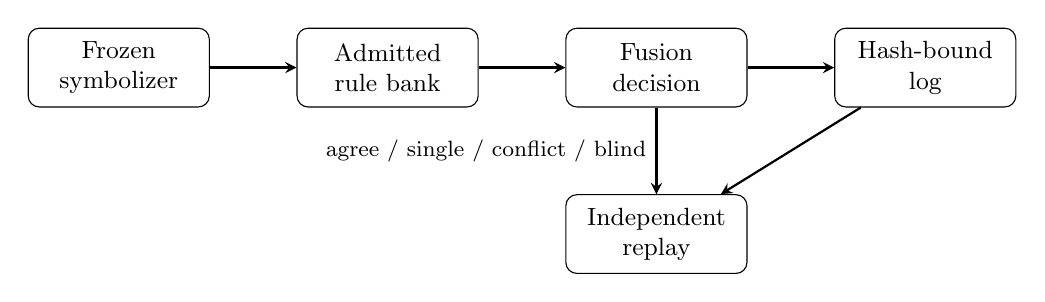
\begin{tikzpicture}[
  node distance=1.1cm, auto,
  block/.style={rectangle, draw, rounded corners, align=center,
    minimum width=2.3cm, minimum height=1.0cm, font=\small},
  arrow/.style={->, >=stealth, thick}]
  \node[block] (cal) {Frozen\\symbolizer};
  \node[block, right=of cal] (bank) {Admitted\\rule bank};
  \node[block, right=of bank] (fuse) {Fusion\\decision};
  \node[block, right=of fuse] (chain) {Hash-bound\\log};
  \node[block, below=of fuse] (replay) {Independent\\replay};
  \draw[arrow] (cal) -- (bank);
  \draw[arrow] (bank) -- (fuse);
  \draw[arrow] (fuse) -- (chain);
  \draw[arrow] (chain) -- (replay);
  \draw[arrow] (fuse) -- node[left, font=\footnotesize]
    {agree / single / conflict / blind} (replay);
\end{tikzpicture}
\caption{Scientific surface of the workflow. Calibration, admission, auditable
selection, binding, and independent replay are separate stages with separate
estimators. Operator steps beyond these five are retained outside the
manuscript. Measured quantities are distinct from schematic quantities
throughout.}
\label{fig:workflow}
\end{figure}

\begin{figure}[t]
\centering
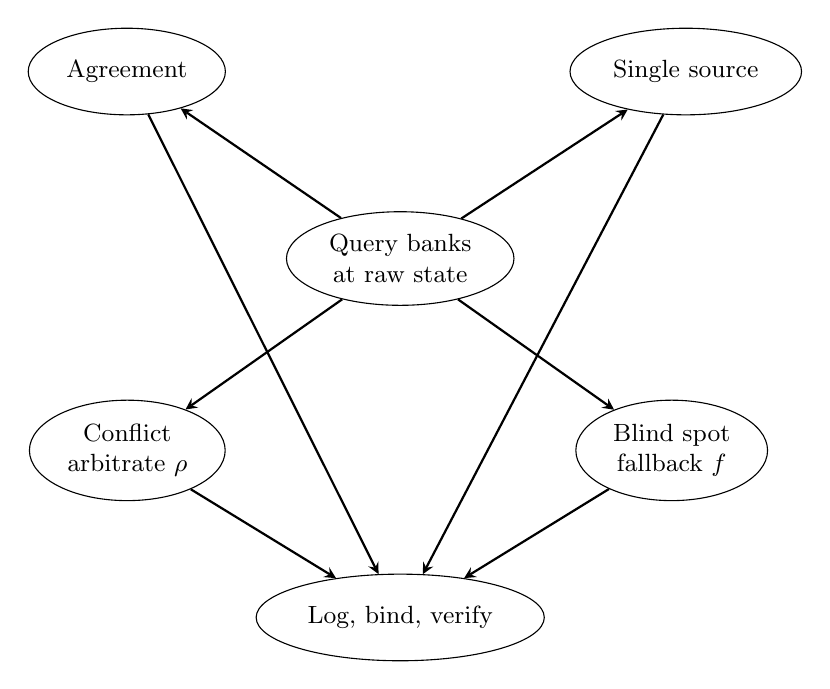
\begin{tikzpicture}[
  node distance=2.2cm, auto,
  state/.style={ellipse, draw, align=center, minimum width=2.4cm,
    minimum height=1.1cm, font=\small},
  arrow/.style={->, >=stealth, thick}]
  \node[state] (q) {Query banks\\at raw state};
  \node[state, above left=of q] (ag) {Agreement};
  \node[state, above right=of q] (sg) {Single source};
  \node[state, below left=of q] (cf) {Conflict\\arbitrate $\rho$};
  \node[state, below right=of q] (bl) {Blind spot\\fallback $f$};
  \node[state, below=of q, yshift=-1.2cm] (lg) {Log, bind, verify};
  \draw[arrow] (q) -- (ag);
  \draw[arrow] (q) -- (sg);
  \draw[arrow] (q) -- (cf);
  \draw[arrow] (q) -- (bl);
  \draw[arrow] (ag) -- (lg);
  \draw[arrow] (sg) -- (lg);
  \draw[arrow] (cf) -- (lg);
  \draw[arrow] (bl) -- (lg);
\end{tikzpicture}
\caption{Fusion decision states. Every deployed action exits through exactly
one of four non-terminal states into a bound, verifiable log entry. Omitted
operator edges are named in the internal audit package.}
\label{fig:fsm}
\end{figure}

\end{document}
